%%%%%%%%%%%%%%%%%%%%%%%%%%%%%%%%%%%%%%%%%%%%%%%%%%%%%%%%%%%%%%%%%%%%%%%%%%%%%%%
%%%%%%%%%%%%%%%%%%%%%%%%%%%%%%%%%%%%%%%%%%%%%%%%%%%%%%%%%%%%%%%%%%%%%%%%%%%%%%%
%%
%%
%%             c.     R  E  S  O  U  R  C  E  S 
%%
%%
%%%%%%%%%%%%%%%%%%%%%%%%%%%%%%%%%%%%%%%%%%%%%%%%%%%%%%%%%%%%%%%%%%%%%%%%%%%%%%%
%%%%%%%%%%%%%%%%%%%%%%%%%%%%%%%%%%%%%%%%%%%%%%%%%%%%%%%%%%%%%%%%%%%%%%%%%%%%%%%
\section{Resources (including project costs)}
Here we summarize and justify the budget.

\begin{figure}
  \begin{center}
    \hspace{-0.5cm}
    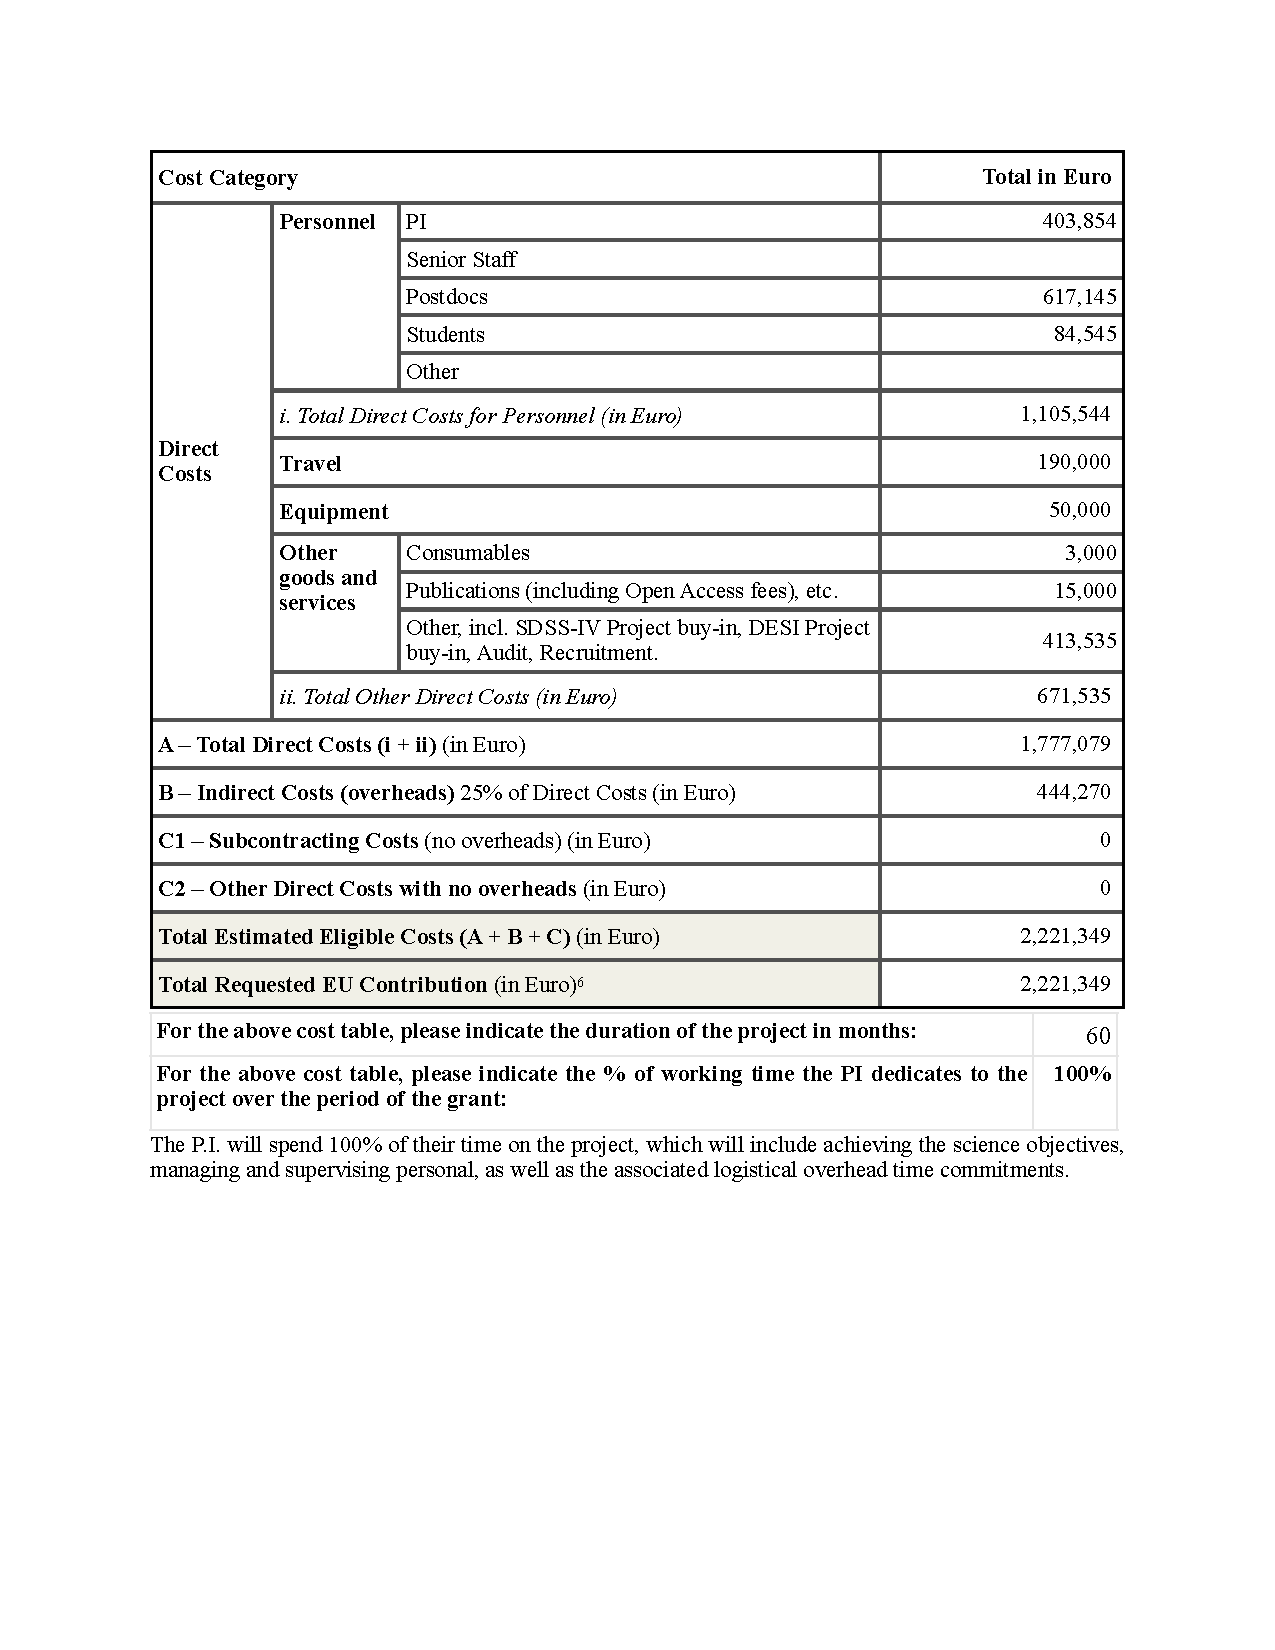
\includegraphics[width=16.6cm]
    {figures/ResourcesSummary.pdf}
    \vspace{-26pt}
 \label{fig:ResourcesSummary}
\end{center}
\end{figure}


\smallskip
\smallskip
\noindent
\textbf{\textsc{Team Composition:}}
Our team will consist of the PI, three postdoctoral research
associates (PDRAs), and 1 PhD student.  Two postdoctoral appointments
will be for three years each and one will be for a four year
appointment (a total of 10 FTE over 5 years).  The PhD student
will have a four year appointment.  The ambitious nature of this
project requires a large team of both observational and theoretical
postdoctoral scholars and PhD students to complete the proposed
research.  The PI is not a current member of academic staff and
therefore has no responsibilities extending beyond research.  As such,
the PI requests 100\% of his salary and, if successful, will focus solely on
the aims of the project.  Again, this will be necessary to achieve all
our goals on the given schedule.

\smallskip
\smallskip
\noindent
NPR is a world-leader in the field of extragalactic observational
astrophysics. NPR's research focuses on implementing novel data
science and machine learning algorithms and techniques in order to
discover and study the physical processes in quasars. I have an
exceptionally strong track record including being the lead of a
science Working Group, with prodigious scientific output
(\href{https://tinyurl.com/ycxd8lb6}{over 400 published, peer-reviewed
papers} from that particular collaboration).

\smallskip
\smallskip
\noindent
I was the Co-Founder and Chief Data Scientist of String Security
Inc. I built a predictive threat detection and remediation
platform for cyber security teams by applying machine learning and
predictive algorithms.  Thus the PI's research strengths, ability to
quickly develop bleeding-edge software and science output are all
ideally matched to this proposal.

\smallskip
\smallskip
\noindent
The skill set of PDRA1 would include development of the underlying
tools and techniques necessary to extract meaning from large and/or
complex data sets.  PDRA1 would have a strong physical sciences
background, and a PhD in astrophysics or computer science.  The skill
sets of PDRA2 would include expertise in time series analysis,
primarily with optical data but potentially also in other wavebands.
PDRA2 would have a PhD in astrophysics or a related field.  The skill
set of PDRA3 would include experience with fluid mechanics modelling
and/or large computer simulations.  PDRA3 would have a PhD in
astrophysics, mathematics or computer science.  PhD1 would have a
Masters or a strong 4-year undergraduate degree in Physics or
Mathematics with evidence of research-level project work.

\smallskip 
\smallskip
\noindent \textbf{\textsc{Salaries:}} The primary expenditure of our
project corresponds to salaries in order support the large team
necessary for this project.  The PI will be fully involved (project
management, scientific analysis, student supervision, postdoc
mentorship, proposal writing, communication with external
collaborations, and paper writing) and is covered at the 100\% level
over 5 years.  Salaries are determined according to the UEDIN salary
scale: \euro80.7k per FTE for the PI, \euro61.3k per FTE for the
PDRAs and \euro21.1k per FTE for PhD students.  The total cost of
salaries over 5 years is {\bf \euro 1106k}.

\smallskip 
\smallskip
\noindent \textbf{\textsc{Travel and Communication:}} 
A major expense is in the form of travel. I expect all group members
to disseminate our results in international conference but also to
participate in external collaboration meeting (at least one per year).
I am currently tax-payer funded, and a deep believer in letting
citizens know how their governments spend public money when investing
in scientific projects with potential impact on their lives and on
society.  Thus broad communication of this research project is a large
personal goal. Due to the nature and timing of our proposal, it will
almost certainly be critical for the PDRAs to have extended (several
week long) visits to the US and ESO Chile. I have allocated thus
allocated \euro10k/year for all members of the group for travel. This
level of commitment is necessary as has been proved by the PI's recent
and continued involvement with the e.g.  US-based surveys (and the
benefit to his research fellowship). The total travel budget is {\bf
\euro190k.}

\smallskip
\smallskip
\noindent
\textbf{\textsc{Publications:}}
Our work will be published in international journals such as Nature,
Nature Astronomy, Science, Monthly Notices of the Royal Astronomical
Society and the Astrophysical Journal. I have allocated \euro3k/year
for the cost of publications. In addition, all papers will be on the
arXiv preprint server free of charge. The total publications budget is
{\bf \euro15k.}

\smallskip
\smallskip
\noindent
\textbf{\textsc{Equipment \& Consumables:}} I have allocated
\euro10k/person for the initial purchase of a desktop and laptop
computer.  While we will have adequate resources to fully deploy {\tt
QuasarSieve} and will run our theory simulations on institute
(e.g. IfA Cullen), university
(e.g. \href{https://www.ed.ac.uk/information-services/research-support/research-computing/ecdf}{Edinburgh
Compute and Data Facility}) or national
{\href{https://www.hartree.stfc.ac.uk/Pages/home.aspx}{(The Hartree
Centre)} facilites, the rate limiting factor of our project and WPs
will be how quickly and efficiently we can deploy our new codes and
analysis.

\smallskip \smallskip
\noindent We require the budget for mid-to-high end hardware, (with
specifications that are not in the typical desktop the university
would supply) and also the e.g. large format displays that massively
boost productivity.  This can include having more than one
monitor 
(
%most programmers agree, and having experience this for myself, having 
e.g. 2 monitors leads to efficient coding, giving 
one full, often `portrait' monitor for code, and another for
documentation, specifications, StackOverflow help etc.)
Laptops are necessary for any extended time away (e.g. ``First Light' travel 
justified above) from the office. 
%\smallskip \smallskip \noindent 
Consumables are limited to \euro600/year (for the purchase
of back-up drives and other equipment). The total equipment and
consumables budget is {\bf \euro53k.}



\smallskip
\smallskip
\noindent
\textbf{\textsc{Access to Large Facilities:}}
We ask for additional funds that are available to cover ``access to
large facilities''.  We request support for the ``buy-in'' to two of
the new surveys, SDSS-V and DESI. The costs here are \euro184.1k and
\euro200.1k, respectively.
%%
We specifically request access to these
funds as it gives our project access to telescopes and data in the
North and Southern Hemispheres (for complete coverage of the celestial
sphere) and delivers the crucial early spectroscopy that will be vital
to train, test and build our data science and machine learning codes
and algorithms.  We emphasise that the science return is `exponential'
(rather than `linearly') dependent on the breadth of data available
and heralds a brand new regime of ``several-survey'' or
``multi-mission'' astronomy. 
Buy-in allows the two observational PDRAs along with the PhD student 
to have data access rights here and 
 {\it would place the
PI and the University of Edinburgh as the only group and institute
in the world to be involved in SDSS-V, DESI, 4MOST, LSST and ESA {\it
Euclid} and JWST}.
The total budget for the access to large facilities is {\bf \euro384.2k}.

\smallskip
\smallskip
\noindent
Total budget before facilities costs: \textbf{\underline{\euro 1,741,099}}. \\
Total budget including facilities costs: \textbf{\underline{\euro 2,221,349}}.\\

